\documentclass[a4paper,12pt]{article}

\usepackage{préambule}

\title{Sondage : Taille des pieds}
\author{Mr Golfouse}
\date{}

\renewcommand{\arraystretch}{1.2}

\begin{document}

\maketitle

Notre sondage porte sur la taille des pieds des élèves, un sujet très important !

\subsection*{Résultats}

Nous avons interrogé 25 élèves au total :

\begin{center}
	\begin{tabular}{|l|c|c|c|c|}
		\hline
		Taille des pieds & $22$ & $23$ & $25$ & $26$
		\\ \hline
		Effectif         & $5$  & $3$  & $2$  & $2$
		\\ \hline
	\end{tabular}
\end{center}

\subsection*{Diagramme}

\begin{center}
	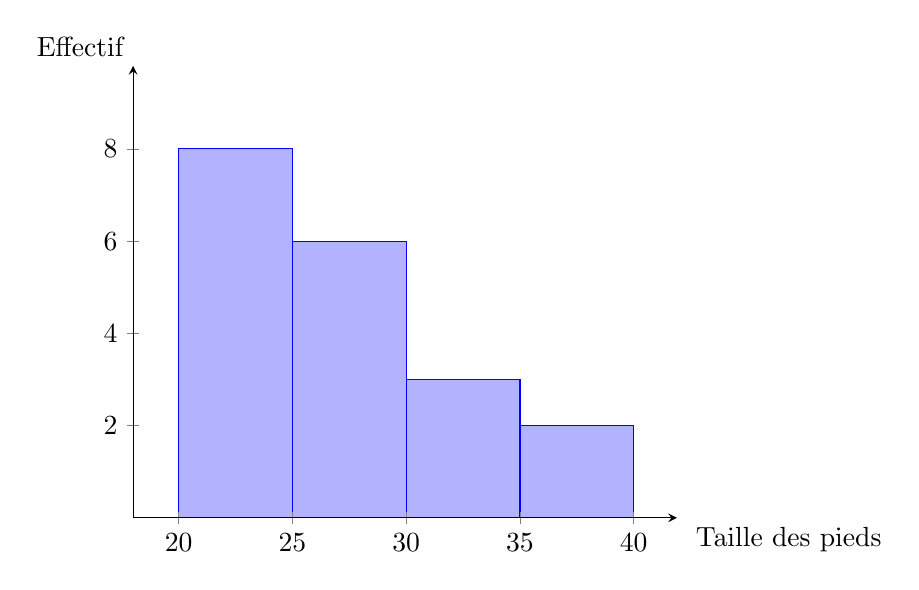
\begin{tikzpicture}
		\begin{axis}[
				width = 0.7\textwidth,
				xmin=18, xmax=41.9,
				ymin=0, ymax=9.8,
				axis lines=center,
				ylabel={Effectif},
				xlabel={\ Taille des pieds},
				xlabel style={below right},
				ylabel style={above left},
				area style,
				xtick=data
			]
			\addplot+[ybar interval,mark=no] plot coordinates { (20,8) (25,6) (30,3) (35,2) (40,2) };
		\end{axis}
	\end{tikzpicture}
\end{center}

\subsection*{Moyenne}

La moyenne des taille de pieds était $30$.

\end{document}